\documentclass[border=5pt]{standalone}
\usepackage{tikz}
\usetikzlibrary{calc,intersections}
\begin{document}
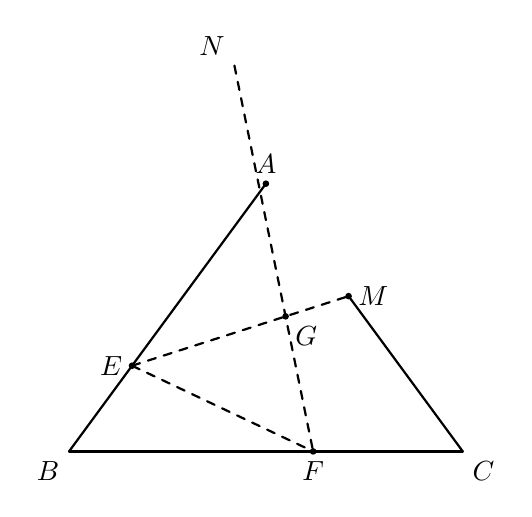
\begin{tikzpicture}[line cap=round,line join=round]
  % 主要坐标
  \coordinate (B) at (0,0);
  \coordinate (C) at (5,0);
  \coordinate (A) at (2.5,3.4);
  \coordinate (E) at ($(B)!0.32!(A)$);
  \coordinate (F) at ($(B)!0.62!(C)$);
  \coordinate (M) at ($(A)!0.42!(C)$);
  \coordinate (N) at (2.1,4.9);
  % 虚线交点 G
  \coordinate (G) at (intersection of E--M and N--F);

  % 实线（删除 AM 的笔画：只画 C 到 M 段）
  \draw[thick] (B) -- (C);
  \draw[thick] (B) -- (A);
  \draw[thick] (C) -- (M);

  % 虚线
  \draw[dashed,thick] (E) -- (M);
  \draw[dashed,thick] (E) -- (F);
  \draw[dashed,thick] (N) -- (F);

  % 点（保留 A、M 的位置）
  \fill (A) circle (1.2pt);
  \fill (M) circle (1.2pt);
  \fill (E) circle (1.2pt);
  \fill (F) circle (1.2pt);
  \fill (G) circle (1.2pt);

  % 标签
  \node[below left] at (B) {$B$};
  \node[below] at (F) {$F$};
  \node[below right] at (C) {$C$};
  \node[left] at (E) {$E$};
  \node[right] at (M) {$M$};
  \node[above] at (A) {$A$};
  \node[above left] at (N) {$N$};
  \node[below right] at (G) {$G$};
\end{tikzpicture}
\end{document}
